% Transcription littérale du TD 08.
% Les abréviations et l'ordre des raisonnements de la copie sont conservés.

\exercise{19}{}

\begin{statementbox}
Lundi 9 Novembre 2026

19| On dit qu'un anneau $A$ (intègre, commutatif) est euclidien ssi $\exists v : A \setminus \{0\} \to \N / \forall (a,b) \in A \times (A \setminus \{0\}), \exists (q,r) \in A^2 / a = bq + r$ avec $\begin{cases} r = 0 \\ \text{ou } v(r) < v(b) \end{cases}$
\begin{enumerate}[label=\alph*)]
  \item Donner des exemples
  \item Mq un anneau euclidien est principal
  \item Mq $\Z[i] := \{a+ib \mid (a,b) \in \Z^2\}$ est euclidien [On justifiera que $\forall z = x+iy \in \C, \exists (a,b) \in \Z^2 / |x-a| \leq \frac{1}{2}, |y-b| \leq \frac{1}{2} \text{ et } |z-(a+ib)| < 1$].
\end{enumerate}
\end{statementbox}

\begin{solution}
\partanswer{a)}
$\cdot$ $\Z$ muni de $|\cdot|$
\[ \forall (a,b) \in \Z \times \Z^*, \exists (q,r) \in \Z^2 / a = bq + r \text{ avec } r \in \llbracket 0, |b|-1 \rrbracket \]
Par division euclidienne de $a$ par $b$.

$\cdot$ $\mathbb{K}[X]$ muni de $\deg$
\[ \forall (A,B) \in \mathbb{K}[X] \times (\mathbb{K}[X] \setminus \{0\}), \exists (Q,R) \in \mathbb{K}[X]^2 / A = BQ + R \text{ avec } \begin{cases} R = 0 \\ \text{ou } \deg R < \deg B \end{cases} \]

\partanswer{b)}
Soit $A$ un anneau euclidien.
Soit $I$ un idéal $\neq \{0\}$ de $A$.
Soit $n_0 := \min \{v(x) / x \in I \setminus \{0\}\}$ et $x_0 \in I \setminus \{0\} / v(x_0) = n_0$.
Comme $I$ est un idéal, $x_0 A \subset I$.
\begin{itemize}
  \item Soit $x \in I$ ; $\exists (q,r) \in A^2 / x = x_0 q + r$ avec $\begin{cases} r = 0 \\ \text{ou } v(r) < v(x_0) \end{cases}$
\end{itemize}
Il vient $r = \underbrace{x - x_0 q}_{\in I}$ (car $x_0 q \in I$ et $I$ sous-groupe additif).
Si $r \neq 0$, $v(r) < n_0$, ce qui ne se peut.
Donc $r = 0$ et $x = x_0 q$. Donc $I = x_0 A$.
$A$ est un anneau principal.

\partanswer{c)}
\textbf{Lemme :} Soit $x \in \R, \exists a \in \Z, |x-a| \leq \frac{1}{2}$. \\
\textbf{Dém :} Si $x \in \left[\lfloor x \rfloor, \lfloor x \rfloor + \frac{1}{2}\right]$, soit $a = \lfloor x \rfloor$ ; $0 \leq x - a \leq \frac{1}{2}$. \\
Si $x \in \left[\lfloor x \rfloor + \frac{1}{2}, \lfloor x \rfloor + 1\right[$, soit $a = \lfloor x \rfloor + 1$ ; $0 < a - x \leq \frac{1}{2}$.

\begin{center}
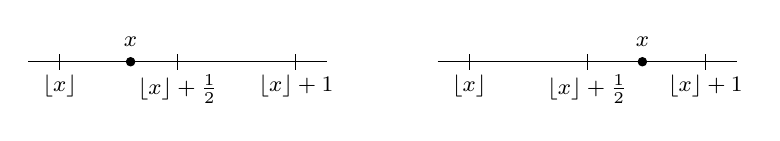
\begin{tikzpicture}[scale=1.0]
  \draw (-0.4,0) -- (3.4,0);
  \draw (0,-0.1) -- (0,0.1) node[below=4pt] {\footnotesize $\lfloor x \rfloor$};
  \draw (1.5,-0.1) -- (1.5,0.1) node[below=4pt] {\footnotesize $\lfloor x \rfloor + \frac{1}{2}$};
  \draw (3,-0.1) -- (3,0.1) node[below=4pt] {\footnotesize $\lfloor x \rfloor + 1$};
  \filldraw (0.9,0) circle (1.5pt) node[above=2pt] {\footnotesize $x$};

  \begin{scope}[xshift=5.2cm]
    \draw (-0.4,0) -- (3.4,0);
    \draw (0,-0.1) -- (0,0.1) node[below=4pt] {\footnotesize $\lfloor x \rfloor$};
    \draw (1.5,-0.1) -- (1.5,0.1) node[below=4pt] {\footnotesize $\lfloor x \rfloor + \frac{1}{2}$};
    \draw (3,-0.1) -- (3,0.1) node[below=4pt] {\footnotesize $\lfloor x \rfloor + 1$};
    \filldraw (2.2,0) circle (1.5pt) node[above=2pt] {\footnotesize $x$};
  \end{scope}
\end{tikzpicture}
\end{center}

Soit $z = x+iy \in \C, \exists (a,b) \in \Z^2 / \begin{cases} |x-a| \leq \frac{1}{2} \\ |y-b| \leq \frac{1}{2} \end{cases}$ Alors :
\[ |z - (a+ib)| = \sqrt{(x-a)^2 + (y-b)^2} \leq \frac{1}{\sqrt{2}} < 1 \]
On définit $v : \Z[i] \setminus \{0\} \to \N, z = a+ib \mapsto a^2+b^2$.
Soit $z_0 \in \Z[i] \setminus \{0\}, z_1 \in \Z[i]$.
On cherche $(q,r) \in \Z[i]^2 / z_1 = z_0 q + r$ avec $|r|^2 < |z_0|^2$, ssi $\frac{z_1}{z_0} = q + \frac{r}{z_0}$ avec $\left|\frac{r}{z_0}\right| < 1$.
Or $\frac{z_1}{z_0} \in \C$, donc $\exists q \in \Z[i] / \left|\frac{z_1}{z_0} - q\right| < 1$.
Soit $r = z_1 - z_0 q \in \Z[i]$.
On a bien $\left|\frac{r}{z_0}\right| = \left|\frac{z_1}{z_0} - q\right| < 1$.
Ainsi $\Z[i]$ est euclidien donc principal.

\begin{remarkbox}
Rem : Nous avons vu que $\Z[i]^\times = \mathbb{U}_4 = \{1, -1, i, -i\}$.

\begin{center}
\begin{tikzpicture}[scale=1.0]
  \draw[->] (-1.6,0) -- (1.6,0);
  \draw[->] (0,-1.4) -- (0,1.4);
  \filldraw (1,0) circle (1.5pt) node[below right] {\footnotesize $1$};
  \filldraw (-1,0) circle (1.5pt) node[below left] {\footnotesize $-1$};
  \filldraw (0,1) circle (1.5pt) node[above left] {\footnotesize $i$};
  \filldraw (0,-1) circle (1.5pt) node[below right] {\footnotesize $-i$};
  \filldraw (1.2,0.65) circle (1.5pt) node[above right] {\footnotesize $z = a+ib$};
  \draw[->] (0.4,0) arc (0:90:0.4) node[midway, above right=-2pt] {\footnotesize $\pi/2$};
\end{tikzpicture}
\end{center}

$\forall z \in \C^*, \exists! \varepsilon \in \mathbb{U}_4 / \varepsilon z$ vérifie $\operatorname{Re}(\varepsilon z) > 0$ et $\operatorname{Im}(\varepsilon z) \geq 0$.
$A_1 = \{z \in \C / \operatorname{Re} z > 0, \operatorname{Im}(z) \geq 0\}$. \\
Soit $\mathcal{P}_1 = \{\text{irréductibles de } \Z[i] \in A_1\}$. D'après le théorème de factorialité :
\[ \forall z \in \Z[i] \setminus \{0\}, \exists! \varepsilon \in \mathbb{U}_4, \exists! (\nu_p(z))_{p \in \mathcal{P}_1} \in \N^{(\mathcal{P}_1)} \text{ presque nulle } / z = \varepsilon \prod_{p \in \mathcal{P}_1} p^{\nu_p(z)} \]
On vérifie que $\mathcal{P}_1 = \underbrace{\{\text{nombres premiers qui ne sont pas sommes de deux carrés}\}}_{(= \text{nb premiers } \equiv 3 [4])} \cup \{z \in \Z[i] / \operatorname{Re} z > 0, \operatorname{Im}(z) \geq 0 \text{ et } |z|^2 \text{ est premier}\}$ avec $|z|^2 = 2$ ou $|z|^2 \equiv 1 [4]$.
\end{remarkbox}
\end{solution}

\exercise{22}{}

\begin{statementbox}
Soit $p \in \mathbb{P}$, mq $\sum_{k=0}^p \binom{p}{k}\binom{p+k}{k} \equiv 2^p + 1 [p^2]$.
\end{statementbox}

\begin{solution}
\[ \sum_{k=0}^p \binom{p}{k}\binom{p+k}{k} = 1 + \binom{2p}{p} + \sum_{k=1}^{p-1} \binom{p}{k}\binom{p+k}{k} \]
or $\forall k \in \llbracket 1, p-1 \rrbracket, p \mid \binom{p}{k}$ $\big[$car $k \binom{p}{k} = p \binom{p-1}{k-1}$ et $k \wedge p = 1\big]$.
$\exists \alpha_k \in \N^* / \binom{p}{k} = p \alpha_k$.

Soit alors $\beta_k = \binom{p+k}{k} = \frac{(p+k)!}{k! (p!)} = \frac{(p+k)(p+k-1)\dots(p+1)}{k!}$.
Ainsi $k! \beta_k = (p+k)\dots(p+1)$.
Dans $\mathbb{F}_p$ : $\overline{k!} \cdot \overline{\beta_k} = \overline{k!}$ et $\overline{k!}$ est inversible car $k \in \llbracket 1, p-1 \rrbracket$ (donc $p \nmid k!$).
D'où $\overline{\beta_k} = \overline{1}$ donc $\beta_k \equiv 1 [p]$.
$\exists \gamma_k \in \Z / \beta_k = 1 + p \gamma_k$.
\[ \binom{p}{k}\binom{p+k}{k} = p \alpha_k (1 + p \gamma_k) \equiv p \alpha_k [p^2] \equiv \binom{p}{k} [p^2] \]
Ainsi : $\sum_{k=1}^{p-1} \binom{p}{k}\binom{p+k}{k} \equiv \underbrace{\sum_{k=1}^{p-1} \binom{p}{k}}_{= 2^p - 2} [p^2]$ et $\sum_{k=0}^p \binom{p}{k}\binom{p+k}{k} \equiv \binom{2p}{p} + 2^p - 1 [p^2]$.

Or $\binom{2p}{p} = \frac{(2p)!}{(p!)^2} = \frac{(2p)(2p-1)\dots(p+1)}{p(p-1)! \cdot p!} = 2 \frac{\prod_{k=1}^{p-1} (p+k)}{(p-1)!}$
et
\[ \prod_{k=1}^{p-1} (p+k) \equiv (p-1)! + p \sum_{k=1}^{p-1} \underbrace{\left(\prod_{\substack{i=1 \\ i \neq k}}^{p-1} i\right)}_{\frac{(p-1)!}{k}} [p^2] \]
Ainsi $(p-1)! \binom{2p}{p} \equiv 2 \left[ (p-1)! + p \sum_{k=1}^{p-1} \frac{(p-1)!}{k} \right] [p^2]$.

Montrons que $\sum_{k=1}^{p-1} \frac{(p-1)!}{k} \equiv 0 [p]$ pour $p \geq 3$.
Posons $\forall k \in \llbracket 1, p-1 \rrbracket, \delta_k = \frac{(p-1)!}{k} \in \N$ ; $k \delta_k = (p-1)!$.
Dans $\mathbb{F}_p$ : $\overline{k} \times \overline{\delta_k} = \overline{(p-1)!}$ et $\overline{k}$ est inversible dans $\mathbb{F}_p$ (car $k \in \llbracket 1, p-1 \rrbracket$ donc $k \wedge p = 1$).
Donc $\overline{\delta_k} = \overline{(p-1)!} \times (\overline{k})^{-1}$.
Ainsi, $\sum_{k=1}^{p-1} \overline{\delta_k} = \sum_{k=1}^{p-1} \overline{(p-1)!} \times (\overline{k})^{-1} = \overline{(p-1)!} \times \sum_{k=1}^{p-1} (\overline{k})^{-1}$.

Or $f : \begin{array}[t]{rcl} \mathbb{F}_p^* & \to & \mathbb{F}_p^* \\ \overline{k} & \mapsto & \overline{k}^{-1} \end{array}$ est bijective.
D'où : $\sum_{k=1}^{p-1} (\overline{k})^{-1} = \sum_{k=1}^{p-1} \overline{k} = \overline{\left(\frac{p(p-1)}{2}\right)}$
et $p$ premier $\geq 3$ est impair donc $\frac{p-1}{2} \in \N$. Ainsi $\overline{\left(\frac{p(p-1)}{2}\right)} = \overline{0}$ et $\sum_{k=1}^{p-1} \overline{\delta_k} = \overline{0}$.
Finalement : $\sum_{k=1}^{p-1} \frac{(p-1)!}{k} \equiv 0 [p]$ pour $p \geq 3$, et $(p-1)! \binom{2p}{p} \equiv 2(p-1)! [p^2]$.

Dans $\Z/p^2\Z$ : $\widetilde{(p-1)!}$ est inversible et $\widetilde{(p-1)!} \widetilde{\binom{2p}{p}} = \widetilde{2} \widetilde{(p-1)!}$.
D'où $\widetilde{\binom{2p}{p}} = \widetilde{2}$ et $\binom{2p}{p} \equiv 2 [p^2]$.
Pour $p=2$ : $\binom{4}{2} \equiv 2 [4]$.
En reportant : $\boxed{\sum_{k=0}^p \binom{p}{k}\binom{p+k}{k} \equiv 2^p + 1 [p^2]}$.
\end{solution}

\exercise{27}{}

\begin{statementbox}
Soit $p$ premier $\geq 5$, on définit $H = \mathbb{F}_p \setminus \{\overline{0}, \overline{1}\}$.
\begin{enumerate}[label=\alph*)]
  \item Vérifier qu'on peut écrire et définir $f : \begin{array}[t]{rcl} H & \to & H \\ x & \mapsto & \overline{1} - x^{-1} \end{array}$ et calculer $f \circ f \circ f$ (on pourra remarquer que $\forall x \in H, f(x) = (x - \overline{1})x^{-1}$).
  \item Mq $-\overline{3}$ est un carré dans $\mathbb{F}_p$ ssi $f$ admet (au moins) un point fixe.
  \item Mq $-\overline{3}$ est un carré dans $\mathbb{F}_p$ ssi $p \equiv 1 [3]$ (on pourra décomposer $f$ en produit de cycles de support disjoints).
\end{enumerate}
\end{statementbox}

\begin{solution}
\partanswer{a)}
Soit $x \in H$ :
\begin{itemize}
  \item si $\overline{1} - x^{-1} = \overline{1}$ alors $x^{-1} = \overline{0}$ ce qui ne se peut.
  \item si $\overline{1} - x^{-1} = \overline{0}$ alors $x^{-1} = \overline{1}$ ce qui ne se peut.
\end{itemize}
Donc $f$ est bien définie de $H$ dans $H$, et $\forall x \in H, f(x) = (x - \overline{1})x^{-1}$.
Alors :
\begin{align*}
f(f(x)) &= (f(x) - \overline{1}) f(x)^{-1} \\
&= (f(x) - \overline{1}) \times x (x - \overline{1})^{-1} \\
&= -x^{-1} x (x - \overline{1})^{-1} = (\overline{1} - x)^{-1}
\end{align*}
Et :
\begin{align*}
f \circ f \circ f(x) &= (f^2(x) - \overline{1}) (f^2(x))^{-1} \\
&= ((\overline{1} - x)^{-1} - \overline{1})(\overline{1} - x) \\
&= \overline{1} - (\overline{1} - x) = x
\end{align*}
Ainsi $f \circ f \circ f = \mathrm{id}_H$.

\partanswer{b)}
Soit $y \in H$ ; on a :
\begin{align*}
f(y) = y &\iff \overline{1} - y^{-1} = y \\
&\iff y^2 - y + \overline{1} = \overline{0} \\
&\iff \overline{4}y^2 - \overline{4}y + \overline{4} = \overline{0} \\
&\iff (\overline{2}y - \overline{1})^2 = -\overline{3}
\end{align*}
Si $\exists y \in H / f(y) = y$, en posant $x = \overline{2}y - \overline{1}$ on a $x^2 = -\overline{3}$. \\
Si $\exists x \in \mathbb{F}_p / x^2 = -\overline{3}$, soit $y = (x + \overline{1}) \times \overline{2}^{-1} \neq \overline{0}$ car $x \neq -\overline{1}$ puisque $(-\overline{1})^2 = \overline{1} \neq -\overline{3}$ (et $y \neq \overline{1}$ car $x \neq \overline{1}$).
On a bien $y \in H$ et $f(y) = y$.

\partanswer{c)}
Comme $p$ est premier $\geq 5$, $p > 3$ et $p \equiv 1 \text{ ou } 2 [3]$.
\begin{itemize}
  \item Si $p \equiv 2 [3]$ : $f$ réalise une permutation de $H$ de cardinal $p - 2 \equiv 0 [3]$, et $f^3 = \mathrm{id}_H$ donc les cycles de support disjoints dont $f$ est le produit sont de longueur $1$ ou $3$.
  Or b) mq on a autant de points fixes que de racines de $-\overline{3}$ dans $\mathbb{F}_p$. Comme $\mathbb{F}_p$ est un corps commutatif, $-\overline{3}$ admet au plus deux racines dans $\mathbb{F}_p$.
  Donc $f$ admet au plus $2$ points fixes. Donc $f$ n'admet aucun point fixe (car $|H| \equiv 0 [3]$).
  \item Si $p \equiv 1 [3]$ : $|H| = p - 2 \equiv 2 [3]$ ; il ne peut pas y avoir que des $3$-cycles dans $f$ donc $f$ admet au moins un point fixe.
\end{itemize}
Ex : $p = 19$.
\[ \begin{array}{c|c|c|c|c} x & \overline{1} & \overline{2} & \overline{3} & \overline{4} \\ \hline x^2 & \overline{1} & \overline{4} & \overline{9} & -\overline{3} \end{array} \qquad \overline{4}^2 = -\overline{3} = (-\overline{4})^2 = \overline{15}^2. \]
\end{solution}

\exercise{41}{}

\begin{statementbox}
(ENS) Soit pour $n \in \N^*$, $d(n)$ le nb de diviseurs de $n$.
Mq $\forall \varepsilon > 0, d(n) = \underset{n \to +\infty}{o}(n^\varepsilon)$.
\end{statementbox}

\begin{solution}
Si $n = \prod_{p \in \mathcal{P}} p^{\nu_p(n)}$ avec $\{p \in \mathcal{P} / \nu_p(n) \neq 0\}$ fini,
\[ m = \prod_{p \in \mathcal{P}} p^{\nu_p(m)} \mid n \iff \forall p \in \mathcal{P}, \nu_p(m) \leq \nu_p(n) \iff \forall p \in \mathcal{P}, \nu_p(m) \in \llbracket 0, \nu_p(n) \rrbracket \]
donc $d(n) = \prod_{p \in \mathcal{P}} (\nu_p(n) + 1)$.
Mq $(\ln(d(n)) - \varepsilon \ln(n))_{n \geq 1}$ est majorée. (Suite p. 11)
\end{solution}

\exercise{29}{}

\begin{statementbox}
Trouver les entiers $n \in \N^*$ tq $7 \mid n^n - 3$.
\end{statementbox}

\begin{solution}
Dans $\mathbb{F}_7$ :
si $\overline{n}^n = \overline{3}$, $\overline{3} \in \operatorname{gr}_\times \{\overline{n}\}$. Or $\overline{3}^2 = \overline{2}$ et $\overline{3}^3 = -\overline{1}$, donc $\omega_\times(\overline{3}) = 6$ (car $\omega_\times(\overline{3}) \mid 6$ d'après Lagrange). Ainsi $\overline{n}$ générateur de $(\mathbb{F}_7^*, \times)$, or nb générateurs $\to \varphi(6)$ ($\mathbb{F}_7^*$ gpe cyclique de cardinal $6$) $= 2$.
\[ f : \begin{array}[t]{rcl} (\Z/6\Z, +) & \to & (\mathbb{F}_7^*, \times) \\ \tilde{k} & \mapsto & \overline{3}^k \end{array} \]
est un isomorphisme. Les générateurs de $\Z/6\Z$ sont $\{\tilde{1}, \tilde{5}\}$, donc ceux de $\mathbb{F}_7^*$ sont $\overline{3}$ et $\overline{5}$.
\begin{itemize}
  \item Si $\overline{n} = \overline{3}$ : $\overline{n}^n = \overline{3}^n = \overline{3}$ ssi $6$ divise $(n-1)$, donc $n \equiv 1 [6]$ et $n \equiv 3 [7] \xrightarrow{\text{Th chinois}} n \equiv 31 [42]^*$.
  \item Si $\overline{n} = \overline{5}$ : $\overline{n}^n = \overline{3}$ ssi $\overline{5}^n = \overline{3} = \overline{5}^5$ ssi $\overline{5}^{n-5} = \overline{1}$ ssi $n \equiv 5 [6]$, et $n \equiv 5 [7] \xrightarrow{\text{Th chinois}} n \equiv 5 [42]^*$.
\end{itemize}
Finalement $7 \mid n^n - 3$ ssi $\boxed{n \equiv 31 [42] \text{ ou } n \equiv 5 [42]}$ ($^*$ À la main).
\end{solution}

\exercise{36}{}

\begin{statementbox}
Soit $p \in \mathbb{P}, p \geq 5$, $H_{p-1} = \frac{a}{(p-1)!}$. Mq $p^2 \mid a$.
\end{statementbox}

\begin{solution}
(Déjà $p \mid a$ en effet :
\[ a = (p-1)! H_{p-1} = \sum_{k=1}^{p-1} \frac{(p-1)!}{k} = \sum_{k=1}^{p-1} \alpha_k \]
on a $\overline{k \alpha_k} = \overline{(p-1)!}$ or $\overline{k} \neq \overline{0}$, donc $\overline{\alpha_k} = \overline{(p-1)!} \overline{k}^{-1}$ et puisque $\overline{k} \mapsto \overline{k}^{-1}$ bijectif :
\[ \sum_{k=1}^{p-1} \overline{\alpha_k} = \sum_{k=1}^{p-1} \overline{(p-1)!} \overline{k} = \overline{(p-1)!} \overline{p} \times \overline{\left(\frac{p-1}{2}\right)} = \overline{0} \]
d'où $\overline{a} = \overline{0}$ et $p \mid a$.)

Astuce magique de l'espace :
\[ 2a = \sum_{k=1}^{p-1} (p-1)! \left(\frac{1}{k} + \frac{1}{p-k}\right) = \sum_{k=1}^{p-1} (p-1)! \frac{p}{k(p-k)} = p \sum_{k=1}^{p-1} \frac{(p-1)!}{k(p-k)} = p \sum_{k=1}^{p-1} \beta_k, \quad \beta_k \in \N \]
on a $k(p-k)\beta_k = (p-1)!$ donc ds $\mathbb{F}_p$ :
\[ -\overline{k}^2 \overline{\beta_k} = \overline{(p-1)!} \quad \text{d'où} \quad \sum_{k=1}^{p-1} \overline{\beta_k} = -\overline{(p-1)!} \sum_{k=1}^{p-1} (\overline{k}^2)^{-1} \]
or $\begin{array}[t]{rcl} \mathbb{F}_p^* & \to & \mathbb{F}_p^* \\ \overline{k} & \mapsto & \overline{k}^{-1} \end{array}$ bijective donc :
\[ \sum_{k=1}^{p-1} \overline{\beta_k} = -\overline{(p-1)!} \times \sum_{k=1}^{p-1} \overline{k}^2 = -\overline{(p-1)!} \overline{\left(\frac{p(p-1)(2p-1)}{6}\right)} \]
par $p$ premier $\geq 5$ :
\begin{itemize}
  \item $2 \mid p-1$ donc $2 \mid p(p-1)(2p-1)$
  \item $p \equiv 1 \text{ ou } 2 [3]$ : si $p \equiv 1 [3]$, $3 \mid p-1$ ; si $p \equiv 2 [3]$, $3 \mid 2p-1$.
\end{itemize}
Ds tous les cas $6 \mid p(p-1)(2p-1)$, d'où $\overline{\left(\frac{p(p-1)(2p-1)}{6}\right)} = \overline{0}$.
Ainsi $p \mid \sum_{k=1}^{p-1} \beta_k$ d'où $p^2 \mid 2a$.
Th de Gauss $\to \boxed{p^2 \mid a}$ ($2 \wedge p = 1$).
\end{solution}

\exercise{87}{}

\begin{statementbox}
Soit $n \in \N^*$, $\mathcal{P}_n = \{e^{2ik\pi/n}, k \in \llbracket 1, n \rrbracket, k \wedge n = 1\}$ les racines primitives $n$-ièmes de l'unité.
Soit le $n$-ième polynôme cyclotomique $\Phi_n = \prod_{\xi \in \mathcal{P}_n} (X - \xi)$.
\begin{enumerate}[label=\alph*)]
  \item Mq $X^n - 1 = \prod_{d \mid n} \Phi_d$, en déduire que $\forall n \in \N^*, \Phi_n \in \Z[X]$.
  \item Soit $p \in \mathbb{P}$, on suppose que $\exists a \in \Z / p \mid \Phi_n(a)$ et $\forall d \mid n, d \neq n, p \nmid \Phi_d(a)$. Mq $p \equiv 1 [n]$.
  \item En déduire qu'il existe une infinité de nbs premiers $\equiv 1 [n]$ (Ind : on justifiera que $\forall d \mid n, d \neq n, \exists (U_d, V_d, b_d) \in \Z[X]^2 \times \Z^* / U_d \Phi_n + V_d \Phi_d = b_d$ et on montrera que $\forall P \in \Z[X]$ non constant, $\{p \text{ premiers} / \exists k \in \Z, p \mid P(k)\}$ est infini).
\end{enumerate}
\end{statementbox}

\begin{solution}
\partanswer{a)}
$\mathbb{U}_n = \bigsqcup_{d \mid n} \{z \in \mathbb{U}_n / \omega(z) = d\} = \bigsqcup_{d \mid n} \mathcal{P}_d$ (Th de Lagrange), d'où :
\[ X^n - 1 = \prod_{\xi \in \mathbb{U}_n} (X - \xi) = \prod_{d \mid n} \left(\prod_{\xi \in \mathcal{P}_d} (X - \xi)\right) = \prod_{d \mid n} \Phi_d \]
Par récurrence forte sur $n \in \N^*$. $\Phi_1 = X - 1 \in \Z[X]$.
Soit $n \geq 2$, supposons que $\forall k \in \llbracket 1, n-1 \rrbracket, \Phi_k \in \Z[X]$.
$X^n - 1 = \Phi_n \prod_{\substack{d \mid n \\ d \neq n}} \Phi_d$ donc $\Phi_n = (X^n - 1) \Big/ \prod_{\substack{d \mid n \\ d \neq n}} \Phi_d$. Or $\prod_{\substack{d \mid n \\ d \neq n}} \Phi_d \in \Z[X]$ unitaire, par algorithme de division euclidienne $\Phi_n \in \Z[X]$.

\partanswer{b)}
Par a) dans $\mathbb{F}_p$ : $\overline{a}^n - \overline{1} = \overline{\Phi_n(a)} \times \prod_{\substack{d \mid n \\ d \neq n}} \overline{\Phi_d(a)} = \overline{0}$, d'où $\overline{a}^n = \overline{1}$ et $\omega_\times(\overline{a}) \mid n$.
Si $\omega_\times(\overline{a}) = d \neq n$, on a $\overline{a}^d - \overline{1} = \overline{0} = \prod_{d' \mid d} \overline{\Phi_{d'}(a)}$ ($\neq \overline{0}$ car $d' \mid n$ et $d' \neq n$) ce qui ne se peut.
Donc $\omega_\times(\overline{a}) = n$ et $\overline{a}^{p-1} = \overline{1}$ (petit Fermat), donc $n \mid p-1$ d'où $\boxed{p \equiv 1 [n]}$.

\partanswer{c)}
Soit $d \mid n, d \neq n$, $\Phi_d \wedge \Phi_n = 1$ (aucune racine commune dans $\C$) le pgcd étant indépendant du corps de référence (Euclide) $\Phi_d \wedge \Phi_n = 1$ dans $\mathbb{Q}[X]$. Par le Th de Bézout :
\[ \exists (A,B) \in \mathbb{Q}[X]^2 \quad A \Phi_n + B \Phi_d = 1 \]
En notant $b_d \in \N^*$ le ppcm des dénominateurs de $A$ et $B$, $U_d = b_d A, V_d = b_d B$ sont des polynômes de $\Z[X]$ ; on a $U_d \Phi_n + V_d \Phi_d = b_d$.

\textbf{Lemme :} Soit $P = \alpha_0 + \alpha_1 X + \dots + \alpha_m X^m \in \Z[X]$ non constant $\alpha_m \neq 0$ et $m \geq 1$. Alors $\{p \in \mathbb{P} / \exists a \in \Z, p \mid P(a)\}$ est infini. \\
\textbf{Dém :} Supposons $= \{p_1, \dots, p_N\}$.
\begin{itemize}
  \item Si $\alpha_0 = 0$ : $P = X Q, Q \in \Z[X]$, $\forall p \in \mathbb{P}, p \mid P(p)$.
  \item Si $\alpha_0 \neq 0$ : $P(0) = \alpha_0$, les facteurs $1^{\text{ers}}$ de $\alpha_0 \in \{p_1, \dots, p_N\}$.
  Comme $P$ est non constant, $|P(a)| \sim |\alpha_m a^m| \xrightarrow[|a| \to +\infty]{} +\infty$, $\exists k \in \N^*$, $P(\alpha_0(p_1 \dots p_N)^k) \neq 0$ et :
  \[ P(\alpha_0(p_1 \dots p_N)^k) = \alpha_0 \left(1 + \alpha_1(p_1 \dots p_N)^k + \dots\right) \]
  avec $1 + \alpha_1(p_1 \dots p_N)^k + \dots \equiv 1 [p_i] \; \forall i \in \llbracket 1, N \rrbracket$.
  Donc un facteur premier de $(1 + \alpha_1(p_1 \dots p_N)^k + \dots)$ est différent de tous les $(p_i)$, ce qui ne se peut.
\end{itemize}

Les $(b_d)_{\substack{d \mid n \\ d \neq n}}$ possèdent un nombre fini de facteurs premiers et $\{p \in \mathbb{P} / \exists a \in \Z, p \mid \Phi_n(a)\}$ est infini d'après le Lemme.
Donc $\{p \text{ premier} / \exists a \in \Z, p \mid \Phi_n(a) \text{ et } \forall d \mid n, d \neq n, p \nmid b_d\}$ est infini.
Or si $p \mid \Phi_n(a)$ et $p \nmid b_d$ alors $p \nmid \Phi_d(a)$.
Donc $\{p \in \mathbb{P} / p \equiv 1 [n]\}$ est infini par b).
\end{solution}

\exercise{78}{}

\begin{statementbox}
Soit $P \in \mathbb{Q}[X]$ unitaire de degré $5$ qui admet une racine double sur $\C$. Mq $P$ admet (au moins) une racine rationnelle.
\end{statementbox}

\begin{solution}
On décompose sur $\mathbb{Q}[X]$ :
\[ P = \prod_{\substack{Q \text{ irréductible} \\ \text{unitaire}}} Q^{\nu_P(Q)} \]
$\exists z_0 \in \C, \exists Q_0$ irréductible sur $\mathbb{Q}[X]$ unitaire, $Q_0(z_0) = 0$ et $z_0$ racine double de $P$, $\forall Q \neq Q_0, Q(z_0) \neq 0$. \\
$\hookrightarrow$ (M. Favennec effacé)
\end{solution}

\exercise{18}{}

\begin{statementbox}
(Équation de Pell-Fermat) Soit $E = \{x + y\sqrt{2} \in \R_+^* / x \in \N, y \in \Z \text{ et } x^2 - 2y^2 = 1\}$.
\begin{enumerate}[label=\alph*)]
  \item Mq $E$ est un ss-gpe de $(\R_+^*, \times)$.
  \item Soit $E^+ = E \cap ]1, +\infty[$. Justifier que si $x + y\sqrt{2} \in E^+$, alors $0 < x - y\sqrt{2} < 1$ et $y = \left\lfloor \frac{x}{\sqrt{2}} \right\rfloor$.
  \item En déduire que pour $(x + y\sqrt{2}, x' + y'\sqrt{2}) \in (E^+)^2$, on a $x' + y'\sqrt{2} \leq x + y\sqrt{2}$ ssi $x' \leq x$.
  \item Soit $m_0 := \inf E^+$. Justifier que $m_0 \in E^+$ et calculer sa valeur. En déduire que $E = \{m_0^n ; n \in \Z\}$.
\end{enumerate}
\end{statementbox}

\begin{solution}
\partanswer{a)}
$1 = 1 + 0\sqrt{2} \in E$ et $\forall (x + y\sqrt{2}, x' + y'\sqrt{2}) \in E^2$ :
\[ (x + y\sqrt{2})(x' + y'\sqrt{2}) = \underbrace{xx' + 2yy'}_{> 0} + (xy' + x'y)\sqrt{2} \]
Or, $(x,x') \in \N^2$ et $x^2 - 2y^2 = {x'}^2 - 2{y'}^2 = 1 > 0$.
Donc $x^2 > 2y^2$ et $x > \sqrt{2}|y|$. De même, $x' > \sqrt{2}|y'|$.
D'où $xx' > 2|y||y'| \geq 2yy'$ et $xx' + 2yy' \in \N$.
De plus, $(xx' + 2yy')^2 - 2(xy' + x'y)^2 = (xx')^2 + 4(yy')^2 - 2(xy')^2 - 2(x'y)^2 = (x^2 - 2y^2)({x'}^2 - 2{y'}^2) = 1$.
Ainsi, $(x + y\sqrt{2})(x' + y'\sqrt{2}) \in E$.
Enfin, $(x + y\sqrt{2})(x - y\sqrt{2}) = 1$ pour tout $x + y\sqrt{2} \in E$ (dans ce cas, $x - y\sqrt{2} \in E$).
Donc $E$ est bien un sous-groupe de $(\R_+^*, \times)$.

\partanswer{b)}
Soit $(x + y\sqrt{2}) \in E^+$. $x - y\sqrt{2} = \frac{1}{x + y\sqrt{2}} \in ]0, 1[$.
Alors $0 < \frac{x}{\sqrt{2}} - y < \frac{1}{\sqrt{2}} < 1$ donc $y = \left\lfloor \frac{x}{\sqrt{2}} \right\rfloor$.

\partanswer{c)}
Soit $(x + y\sqrt{2}, x' + y'\sqrt{2}) \in (E^+)^2$.
\begin{itemize}
  \item Si $x' \leq x$ : $\left\lfloor \frac{x'}{\sqrt{2}} \right\rfloor = y' \leq \left\lfloor \frac{x}{\sqrt{2}} \right\rfloor = y$. D'où $x' + y'\sqrt{2} \leq x + y\sqrt{2}$.
  \item Si $x' > x$ : $\left\lfloor \frac{x'}{\sqrt{2}} \right\rfloor = y' \geq \left\lfloor \frac{x}{\sqrt{2}} \right\rfloor = y$. D'où $x' + y'\sqrt{2} > x + y\sqrt{2}$.
\end{itemize}
Ainsi, $x' \leq x$ ssi $x' + y'\sqrt{2} \leq x + y\sqrt{2}$.

\partanswer{d)}
Si $x + y\sqrt{2} \in E^+$, alors $x \in \N^*$ et $y = \left\lfloor \frac{x}{\sqrt{2}} \right\rfloor$.
Notons pour $n \in \N^*$ : $u_n := n + \left\lfloor \frac{n}{\sqrt{2}} \right\rfloor \sqrt{2}$ suite strictement croissante (qui parcourt tout $E^+$) et $u_n \in E^+$ ssi $n^2 - 2\left\lfloor \frac{n}{\sqrt{2}} \right\rfloor^2 = 1$ :
\begin{itemize}
  \item $u_1 = 1 \notin E^+$
  \item $u_2 = 2 + \sqrt{2} \notin E^+$ car $2^2 - 2 \times 1^2 = 2 \neq 1$
  \item $u_3 = 3 + 2\sqrt{2} \in E^+$ car $3^2 - 2 \times 2^2 = 9 - 8 = 1$
\end{itemize}
Donc $m_0 = u_3 = 3 + 2\sqrt{2}$.
En outre, $\ln E := \{\ln(x + y\sqrt{2}) / x + y\sqrt{2} \in E\}$ est un sous-groupe additif de $\R$ et $\inf(\ln E \cap \R_+^*) = \ln(m_0) > 0$.
On sait alors que $\ln E = \ln(m_0)\Z$.
D'où $\boxed{E = \{m_0^n ; n \in \Z\}}$.

\begin{remarkbox}
Rem : $E^+ = \{m_0^n ; n \in \N^*\}$ (suite strictement croissante) $= \{3 + 2\sqrt{2}, 17 + 12\sqrt{2}, \dots\}$ avec
\[ m_0^n = (3 + 2\sqrt{2})^n = \sum_{k=0}^n \binom{n}{k} (2\sqrt{2})^k 3^{n-k} = \underbrace{\sum_{k=0}^{\lfloor n/2 \rfloor} \binom{n}{2k} 2^{3k} 3^{n-2k}}_{\in \N} + \sqrt{2} \underbrace{\sum_{k=0}^{\lfloor \frac{n-1}{2} \rfloor} \binom{n}{2k+1} 2^{3k+1} 3^{n-2k-1}}_{\in \N} \]

Rem : Soit $(x,y) \in \Z^2$. Si $x + y\sqrt{2} > 0$ et $x^2 - 2y^2 = 1$, alors $x - y\sqrt{2} = \frac{1}{x + y\sqrt{2}} > 0$ donc $2x = (x + y\sqrt{2}) + (x - y\sqrt{2}) > 0$ et $x \in \N^*$ : $x + y\sqrt{2} \in E$. \\
Si $x + y\sqrt{2} < 0$ et $x^2 - 2y^2 = 1$ : $-(x + y\sqrt{2}) \in E$.
\end{remarkbox}
\end{solution}

\exercise{37}{}

\begin{statementbox}
[À RETENIR] Soit $p$ premier $\geq 3$.
\begin{enumerate}[label=\alph*)]
  \item Mq il y a exactement $\frac{p-1}{2}$ carrés dans $\mathbb{F}_p^*$ (on formera $f : \begin{array}[t]{rcl} \mathbb{F}_p^* & \to & \mathbb{F}_p^* \\ x & \mapsto & x^2 \end{array}$ et on vérifiera que chaque image possède exactement $2$ antécédents).
  \item Soit $x \in \mathbb{F}_p^*$. Mq $x$ est un carré dans $\mathbb{F}_p^*$ ssi $x^{\frac{p-1}{2}} = \overline{1}$.
  \item Mq $-\overline{1}$ est un carré dans $\mathbb{F}_p^*$ ssi $p \equiv 1 [4]$. En déduire qu'il existe une infinité de nombres premiers $\equiv 1 [4]$.
\end{enumerate}
\end{statementbox}

\begin{solution}
\partanswer{a)}
Soit $f : \begin{array}[t]{rcl} \mathbb{F}_p^* & \to & \mathbb{F}_p^* \\ x & \mapsto & x^2 \end{array}$ et $y \in \operatorname{Im}(f)$.
Alors $\exists x \in \mathbb{F}_p^* / x^2 = y$. Soit $x' \in \mathbb{F}_p^*$, $f(x') = y$ ssi $(x - x')(x + x') = \overline{0}$ ssi $x' \in \{-x, x\}$ par intégrité de $\mathbb{F}_p$. De plus, $x \neq \overline{0}$ et $p \geq 3$ (soit $\overline{2} \neq \overline{0}$), donc $x \neq -x$.
Donc chaque image possède exactement $2$ antécédents.
Ainsi, $2 |\operatorname{Im} f| = |\mathbb{F}_p^*| = p - 1$ et $|\operatorname{Im} f| = \frac{p-1}{2}$.

\partanswer{b)}
Si $x$ est un carré, alors $\exists a \in \mathbb{F}_p^* / x = a^2$.
Donc $x^{\frac{p-1}{2}} = a^{p-1} = \overline{1}$ (petit théorème de Fermat). \\
$\big[f$ est un morphisme de groupes et $\operatorname{Im} f$ est un sous-groupe de $\mathbb{F}_p^*$ de cardinal $\frac{p-1}{2} \longrightarrow$ Théorème de Lagrange$\big]$
Le polynôme $X^{\frac{p-1}{2}} - \overline{1}$ admet au plus $\frac{p-1}{2}$ racines car $\mathbb{F}_p$ est un corps.
Ainsi, $x$ est un carré dans $\mathbb{F}_p^*$ ssi $x^{\frac{p-1}{2}} = \overline{1}$.

\partanswer{c)}
$-\overline{1}$ est un carré ssi $(-\overline{1})^{\frac{p-1}{2}} = \overline{1}$ ssi $\frac{p-1}{2}$ pair ssi $p \equiv 1 [4]$.
Si $\{p \text{ premier } \equiv 1 [4]\}$ est fini, notons-le $\{p_1, \dots, p_N\}$.
Considérons $p$ facteur premier de $(p_1 \dots p_N)^2 + 1$ ($> 1$ car $5 \equiv 1 [4]$).
Dans $\mathbb{F}_p$ : $\overline{(p_1 \dots p_N)}^2 + \overline{1} = \overline{0}$ et $-\overline{1}$ est un carré dans $\mathbb{F}_p^*$.
Donc $p \equiv 1 [4]$ donc $p \in \{p_1, \dots, p_N\}$ ce qui ne se peut car $\forall i \in \llbracket 1, N \rrbracket, (p_1 \dots p_N)^2 + 1 \equiv 1 [p_i]$.

\begin{remarkbox}
Rem : Supposons qu'il existe un nb fini $q_1 = 3 < q_2 = 7 < \dots < q_N$ de nbs premiers $\equiv 3 [4]$. Si tous les facteurs premiers de $4 q_2 \dots q_N + 3$ étaient $\equiv 1 [4]$, alors leur produit serait $\equiv 1 [4]$ ce qui ne se peut.
Comme ces facteurs premiers sont impairs, $\exists p$ premier $\equiv 3 [4]$ qui divise $4(q_2 \dots q_N) + 3$ et $\exists i \in \llbracket 1, N \rrbracket / p = q_i$ et $p \neq 3$ car $4 q_2 \dots q_N + 3 \equiv 4(q_2 \dots q_N) \not\equiv 0 [3]$, donc $i \geq 2$ mais $4 q_2 \dots q_N + 3 \equiv 3 [q_i] \not\equiv 0 [q_i]$.
C'est impossible. Donc il y a une infinité de nbs premiers $\equiv 3 [4]$.
\end{remarkbox}
\end{solution}

\exercise{45}{}

\begin{statementbox}
Pour $p$ premier et $r = \frac{a}{b} \in \mathbb{Q}^*$, on définit $\nu_p(r) := \nu_p(a) - \nu_p(b)$.
On a $\forall (r,r') \in (\mathbb{Q}^*)^2, \nu_p(rr') = \nu_p(r) + \nu_p(r')$ et $|r| = \prod_{p \in \mathcal{P}} p^{\nu_p(r)}$.
\begin{enumerate}
  \item Soit $P \in \mathbb{Q}[X] \setminus \{0\}, P = a_0 + a_1 X + \dots + a_n X^n$ avec $n \in \N, a_n \neq 0$. Justifier que $\exists! (c, P_1) \in \mathbb{Q}_+^* \times \Z[X] / P = c P_1$ et que pour $P_1 = \sum_{i=0}^n a'_i X^i, \bigwedge_{i=0}^n a'_i = 1$.
  \item Soit $(P_1, Q_1) \in (\Z[X] \setminus \{0\})^2$ dont les coefficients sont premiers entre eux dans leur ensemble. Mq c'est le cas pour $P_1 Q_1$ [pour $p$ premier on considérera $\forall A = \sum \alpha_i X^i, \overline{A} = \sum \overline{\alpha_i} X^i$ dans $\mathbb{F}_p[X]$ et on vérifiera que si $p$ divise les coeffs de $P_1 Q_1$, il divise ceux de $P_1$ ou ceux de $Q_1$].
  \item Mq $c(PQ) = c(P)c(Q)$.
\end{enumerate}
\end{statementbox}

\begin{solution}
\partanswer{1)}
Supposons l'existence de $c$ et $P_1$. Il vient : $\forall i \in \llbracket 0, n \rrbracket, a_i = c a'_i$.
Soit $p$ premier : $\nu_p(a_i) = \nu_p(c) + \underbrace{\nu_p(a'_i)}_{\geq 0 \text{ car } a'_i \in \Z}$.
Donc $\nu_p(c) \leq \nu_p(a_i) \; \forall i \in \llbracket 0, n \rrbracket$.
De plus, $\exists i_0 \in \llbracket 0, n \rrbracket / p \nmid a'_{i_0}$ car $\bigwedge_{i=0}^n a'_i = 1$. Alors $\nu_p(a'_{i_0}) = 0$ donc $\nu_p(a_{i_0}) = \nu_p(c)$.
Ainsi, $\nu_p(c) = \min_{i \in \llbracket 0, n \rrbracket} \{\nu_p(a_i)\}$ et
\[ c = \prod_{p \in \mathcal{P}} p^{\min \{\nu_p(a_i) ; i \in \llbracket 0, n \rrbracket\}} ; \qquad P_1 = \frac{P}{c} \]
d'où l'unicité en cas d'existence.

Réciproquement, soient $c$ et $P_1$ ainsi définis.
$\forall p \in \mathcal{P}$, $\nu_p(a'_i) = \nu_p(a_i) - \underbrace{\nu_p(c)}_{\leq \nu_p(a_i) \text{ par déf}} \geq 0$ donc $a'_i \in \Z$.
De plus, $\exists i_0 \in \llbracket 0, n \rrbracket, \nu_p(a_{i_0}) = \nu_p(c)$. Alors $\nu_p(a'_{i_0}) = 0$ i.e. $p \nmid a'_{i_0}$.
Ceci vaut $\forall p$ premier donc $\bigwedge_{i=0}^n a'_i = 1$.

\partanswer{2)}
$P_1 = \sum_{i=0}^n \alpha_i X^i, Q_1 = \sum_{j=0}^m \beta_j X^j$. Soit $p$ premier. Si $p$ divise tous les coefficients de $P_1 Q_1$, alors $\overline{P_1} \overline{Q_1} = \overline{0}$ dans $\mathbb{F}_p[X]$.
Or, $\mathbb{F}_p[X]$ est intègre. D'où $\overline{P_1} = \overline{0}$ ou $\overline{Q_1} = \overline{0}$ ce qui ne se peut.
Ainsi, tous les coeffs de $P_1 Q_1$ sont premiers entre eux dans leur ensemble.

\partanswer{3)}
On écrit $PQ = c(P) c(Q) \underbrace{P_1 Q_1}_{\text{coeffs premiers entre eux}}$.
D'où $\boxed{c(PQ) = c(P) c(Q)}$.

\medskip
\textbf{Application :} Trouver tous les $\theta \in [0, \pi] / \frac{\theta}{\pi} \in \mathbb{Q}$ et $\cos \theta \in \mathbb{Q}$ (par ex, $\theta = 0$ ou $\theta = \pi$).

Soit $\theta \in ]0, \pi[$ vérifiant l'hypothèse, $\frac{\theta}{2\pi} \in \mathbb{Q} \cap ]0, \frac{1}{2}[$.
$\exists n \in \N^*, \exists k \in \llbracket 1, n-1 \rrbracket, \frac{\theta}{2\pi} = \frac{k}{n}$ i.e. $\theta = \frac{2k\pi}{n} \in ]0, \pi[$.
Alors $e^{\frac{2ik\pi}{n}} \neq e^{-\frac{2ik\pi}{n}}$ (sinon, $e^{\frac{2ik\pi}{n}} \in \{-1, 1\}$).
Il vient :
\[ X^n - 1 = \left(X - e^{\frac{2ik\pi}{n}}\right)\left(X - e^{-\frac{2ik\pi}{n}}\right) \prod_{\xi \in \mathbb{U}_n \setminus \left\{e^{\frac{2ik\pi}{n}}, e^{-\frac{2ik\pi}{n}}\right\}} (X - \xi) = (X^2 - 2\cos\theta X + 1) \underbrace{B(X)}_{\in \C[X]} \]

\begin{center}
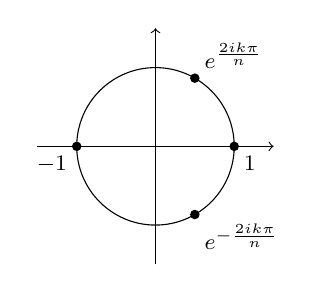
\begin{tikzpicture}[scale=1.0]
  \draw[->] (-1.5,0) -- (1.5,0);
  \draw[->] (0,-1.5) -- (0,1.5);
  \draw (0,0) circle (1cm);
  \filldraw (1,0) circle (1.5pt) node[below right] {\footnotesize $1$};
  \filldraw (-1,0) circle (1.5pt) node[below left] {\footnotesize $-1$};
  \filldraw (60:1) circle (1.5pt) node[above right] {\footnotesize $e^{\frac{2ik\pi}{n}}$};
  \filldraw (-60:1) circle (1.5pt) node[below right] {\footnotesize $e^{-\frac{2ik\pi}{n}}$};
\end{tikzpicture}
\end{center}

On obtient $B$ par division euclidienne de $X^n - 1$ par $X^2 - \underbrace{2\cos\theta}_{\in \mathbb{Q}} X + 1$. L'algorithme d'Euclide prouve que $B \in \mathbb{Q}[X]$.
Soit $A = X^2 - 2\cos\left(\frac{2k\pi}{n}\right)X + 1 \in \mathbb{Q}[X]$.
Or $1 = \underbrace{c(X^n - 1)}_{= 1} = c(A) c(B)$.
Écrivons $A = c(A) A_1$ et $B = c(B) B_1$. Il vient $A \cdot B = \underbrace{c(A) c(B)}_{= 1} A_1 B_1$.
Alors $1 = \operatorname{dom}(X^n - 1) = \underbrace{\operatorname{dom}(A_1)}_{\in \Z} \underbrace{\operatorname{dom}(B_1)}_{\in \Z}$, donc $\operatorname{dom}(A_1) \in \{-1, 1\}$.
Or, $A = c(A) A_1$, d'où $1 = \operatorname{dom}(A) = \underbrace{c(A)}_{\in \mathbb{Q}_+^*} \operatorname{dom}(A_1)$.
Nécessairement, $\operatorname{dom}(A_1) = 1$, d'où $c(A) = 1$ et $A = A_1 \in \Z[X]$.
Donc $2\cos\left(\frac{2k\pi}{n}\right) \in \Z \cap ]-2, 2[ = \{-1, 0, 1\}$.
Donc $\boxed{\theta \in \left\{\frac{\pi}{3}, \frac{\pi}{2}, \frac{2\pi}{3}\right\}}$ (réciproquement ça marche).

\textbf{Ex :} Soit $\theta = \arccos \frac{1}{3}$. Alors $\frac{\theta}{\pi} \notin \mathbb{Q}$. \\
\textbf{Autre preuve :} Si $\theta = \frac{2k\pi}{n}$ alors $\cos(n\theta) = 1 = T_n(\underbrace{\cos\theta}_{= \frac{1}{3}})$, $T_n \in \Z[X]$ de $\mathrm{d}^\circ \, n$ et de coeff dom $2^{n-1}$.
Si $T_n = \alpha_0 + \alpha_1 X + \dots + \alpha_{n-1} X^{n-1} + 2^{n-1} X^n$ :
\[ T_n\left(\frac{1}{3}\right) = \alpha_0 + \frac{\alpha_1}{3} + \dots + \frac{\alpha_{n-1}}{3^{n-1}} + \frac{2^{n-1}}{3^n} = 1 \]
i.e. $3^n \alpha_0 + 3^{n-1}\alpha_1 + \dots + 3\alpha_{n-1} + 2^{n-1} = 3^n$, d'où $3 \mid 2^{n-1}$ ce qui ne se peut.
\end{solution}

\exercise{41 (suite)}{}

\begin{solution}
On note $\forall n \in \N^*, u_n = \ln(d(n)) - \varepsilon \ln(n)$.
Il vient :
\[ u_n = \sum_{p \in \mathcal{P}} \bigl(\ln(1 + \nu_p(n)) - \varepsilon \nu_p(n) \ln(p)\bigr) \]
Or, $\forall p \in \mathcal{P}$,
\[ \ln(1 + \nu_p(n)) - \varepsilon \nu_p(n) \ln(p) \leq (1 - \varepsilon \ln(p)) \underbrace{\nu_p(n)}_{\in \N} \]
$\varepsilon > 0$ étant fixé, $\lim_{p \to +\infty} 1 - \varepsilon \ln(p) = -\infty$.
Donc $\exists p_0 \in \mathcal{P} / \forall p \in \mathcal{P}$, si $p \geq p_0$ alors $1 - \varepsilon \ln(p) \leq 0$.
Alors $\forall n \geq 1$,
\[ u_n \leq \sum_{\substack{p \in \mathcal{P} \\ p < p_0}} \bigl(\ln(1 + \nu_p(n)) - \varepsilon \nu_p(n) \ln(p)\bigr) \]
Or $\forall p \in \mathcal{P} \, (p < p_0), \lim_{x \to +\infty} (\ln(1+x) - \varepsilon x \ln(p)) = -\infty$.
Donc $\forall p \in \mathcal{P} \cap \llbracket 1, p_0 - 1 \rrbracket, \exists A_p > 0 / \forall x \geq A_p, \ln(1+x) - \varepsilon x \ln(p) \leq 0$.
Soit $A = \max_{\substack{p \in \mathcal{P} \\ p < p_0}} \lceil A_p \rceil$, $\forall x \geq A, \forall p \in \mathcal{P} \, (p < p_0), \ln(1+x) - \varepsilon x \ln(p) \leq 0$.
Alors $\forall n \geq 1$,
\[ u_n \leq \underbrace{\sum_{\substack{p \in \mathcal{P} \\ p < p_0}} \sum_{k=0}^A |\ln(1+k) - \varepsilon k \ln(p)|}_{\text{indépendant de } n} \]
Ainsi, $(u_n)_n$ est majorée et $\forall \varepsilon > 0, \boxed{d(n) = \underset{n \to +\infty}{o}(n^\varepsilon)}$.

\begin{remarkbox}
Rem : $\forall \varepsilon > 0, \sum_{n \geq 1} \frac{d(n)}{n^{1+\varepsilon}} \text{ CV} \quad \text{car } d(n) = \underset{n \to +\infty}{o}(n^{\varepsilon/2}), \text{ donc } \frac{d(n)}{n^{1+\varepsilon}} = \underset{n \to +\infty}{o}\left(\frac{1}{n^{1+\frac{\varepsilon}{2}}}\right)$.
\end{remarkbox}
\end{solution}
